\documentclass[12pt]{article}
\usepackage{seantex}

\graphicspath{ {./img/} }

% --- Document Info ---
\title{D\&A: Woche 9}
\author{Sean Findlay}
\date{\today}

% --- Start Document ---
\begin{document}

\maketitle

\section{Shortest Paths}

\begin{definition}{Weighted graph}{}
    A \textbf{weighted graph} $G = (V, E, c)$ is a graph $G = (V, E)$ (where $V$ is the set of vertices (corner points), and $E$ is the set of edges), with a weight function $c: E \rightarrow \R$ that assigns each edge in $E$ a weight.

    We call $c(e)$ the \textbf{weight} (sometimes also the cost) of the edge $e$.
\end{definition}

\begin{figure}[h] % [h] attempts to place the image "here"
    \centering
    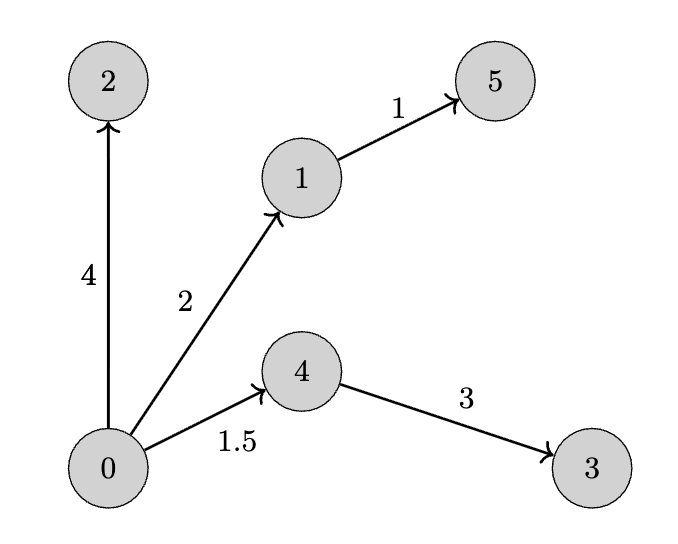
\includegraphics[scale=0.7]{weighted_graph.png}
    \caption{An example of a weighted graph.}
    \label{fig:weighted_graph}
\end{figure}

\begin{remark}{Weight of a path}{}
    Given a weighted graph, we can study the weight of a path. Let us consider a path $p$ from $s$ to $t$. The weight of $p$ is defined as the sum of the weights of its edges:
    $$
        c(p) := \sum_{i = 1}^{k} c((v_i, v_{i+1}))
    $$
\end{remark}

\begin{remark}{Notation for paths}{}
    We usually write $p : s \rightsquigarrow t$ or $s \overset{p}{\rightsquigarrow} t$ to indicate that $p$ is a path from $s$ to $t$, especially when the intermediate nodes do not matter that much.
\end{remark}

\begin{definition}{Shortest path}{}
    The shortest path in a weighted graph $G$ from node $s$ to node $t$ is defined as the path $p$ with minimum weight $\delta(s, t)$, where
    $$
        \delta(s, t) = \begin{cases}
            \infty & \text{no path from } s \text{ to } t \\
            \min\left\{c(p) : s \overset{p}\rightsquigarrow t\right\} & \text{otherwise}
        \end{cases}
    $$

    Note that the shortest path is not always unique. Our goal will be to simply find one shortest path, no matter which one.
\end{definition}

\begin{remark}{Cycles and shortest paths}{}
    A shortest path \textbf{does not} contain any cycles. 
    \begin{itemize}
        \item If the cycle has negative weight (i.e. a cycle such that the total cost of passing through the cycle once is negative), then there exists no shortest path.
        \item If the cycle has positive weight, then the shortest path will not pass through it.
        \item If the cycle has weight zero, then we can omit the cycle without changing the weight of the path. So the shortest path (by convention) does not pass through it.
    \end{itemize}
\end{remark}

\begin{remark}{Shortest paths obey the principle of optimal substructures}{}
    If the shortest path $p$ from $s$ to $t$ goes via a node $v$, then $p$ must contain the shortest path from $s$ to $v$ and the shortest path from $v$ to $t$.

    Formally, if $p = s \overset{p_1}\rightsquigarrow v \overset{p_2}\rightsquigarrow t$, then $p_1$ must be the shortest path from $s$ to $v$ and $p_2$ must be the shortest path from $v$ to $t$.

    More generally, if $p = (v_1, \dots, v_k)$ is a shortest path, then all subpaths $p_{ij}$ for $1 \leq i \leq j \leq k$ are shortest paths as well.
\end{remark}

Due to this observation, computing the shortest paths from a single source $s$ to a target $v$ essentially requires us to compute \textbf{all shortest paths} from a single source to all possible targets in $V$. We thus now consider this more general problem of \textbf{single-source shortest paths}.


\section{Dijkstra's Algorithm}

\begin{warning*}{Important assumption}{}
    From now on, we assume that all weighted graphs have only \textbf{positive} weights.

    We also assume WLOG that there are no edges with weight zero. If there was one, then we can just merge it with one of its neighbouring edges.
\end{warning*}

\begin{notebox}{The problem statement}{}
    We consider the weighted graph $G = (V, E, c)$ with positive weights. We want to find all shortest paths from a source node $s$ to all nodes in $V$.
\end{notebox}

Initially, we know the shortest path from $s$ to $s$. It simply has length $\delta(s, s) = 0$. Next, we can look at the outgoing edges from $s$. The shortest path from $s$ to a neighbouring node $v$ must have a length of at most $c(s, v)$. This provides us with an upper bound.

Now, let us look at the neighbouring node $v$ of $s$ with the smallest upper bound. Could we reach $v$ from $s$ via a path with shorter length than that? No! Because if we could, then $v$ wouldn't be the node with the smallest upper bound. Let us summarise this:

\begin{remark}{}{}
    Let $v$ be the out-neighbour of $s$ with the minimum edge weight, i.e.
    $$
        c(s, v) \leq c(s, w) \ \forall w \in N^+(s)
    $$
    Then, the shortest path from $s$ to $v$ is $c(s, v)$.
\end{remark}

After this, we have found...
\begin{itemize}
    \item the shortest path from $s$ to another node $v$
    \item and we know the upper bounds $d_s[x]$ on$ \delta(s, x)$ for all $x \in N^+(s)$.
\end{itemize}

We can now repeat this process for all outgoing edges of the node $v$ and update the upper bounds of its out-neighbours accordingly. We then have the shortest paths to $s$ and $v$ as well as upper bounds $d_s[\cdot]$ on all nodes in $(N^+(s) \cup N^+(v)) \setminus \{s, v\} $ with $d_s[\cdot] \geq \delta(s, v)$. We note that $d_s[x]$ is the length of the shortest path from $s$ to $x$ that only potentially uses $v$ as an intermediate node, thus $d_s[x]$ is the length of the shorter of $(s, x)$ and $(s, v, x)$.

Let $w$ be the node (different from $s$ and $v$) with the smallest upper bound $d_s[w]$. We can conclude that $d_s[w] = \delta(s, w)$. Why? If there was a better path, it would have to use the cheapest outgoing path from $s$. If another path was cheaper, then this node would be our node with the smallest upper bound (and not $w$). So we ahve found the shortest path to $w$.

\subsection{Formulation of the greedy Dijkstra's algorithm}

\begin{enumerate}
    \item We have a weighted graph $G = (V, E, c)$. Start with $S = \emptyset,\ U = {s},\ R = V \setminus {s}$.
        \begin{itemize}
            \item $S$ is the set with the known shortest path,
            \item $U$ is the set of nodes reachable from $S$ for which we know an upper bound,
            \item $R$ is the set for which we do not know an upper bound (other than $\infty$)
        \end{itemize}
        Repeat the following until $S = V$ and hence $U = \emptyset$
    
        \item In each iteration, we add the node $u$ from $U$ with the \textbf{smallest} upper bound $d_s[u]$ to $S$ and remove it from $U$. We set its shortest path length to $d_s[u]$ and update $d_s$ for all nodes in $N^+(u)$.
        
        More concretely,
        
        \begin{itemize}
            \item If there is an edge $(u, a)$ to a node $a \in S$, then this edge is ignored.
            \item If there is an edge to a node $b \in U$ with $d_s[b] \leq d_s[u] + c((u, b))$, then this edge is ignored.
            \item If there is an edge to a node $c \in U$ with $d_s[c] > d_s[u] + c((u, c))$, then the upper bound of $c$ is updated to $d_s[c] \leftarrow d_s[u] + c((u, c))$.
            \item If there is an edge $(u, d)$ to a node $d \in R$ (a node with no known upper bound), then $d$ is added to $U$ and its upper bound is set to $d_s[d] \leftarrow d_s[u] + c((u, d))$.
        \end{itemize}
\end{enumerate}

After $i$ iterations, we have $|S| = i$. Hence, the algorithm terminates after $n$ iterations and claims to have found the shortest path to all nodes in $V$.

\begin{figure}[h] % [h] attempts to place the image "here"
    \centering
    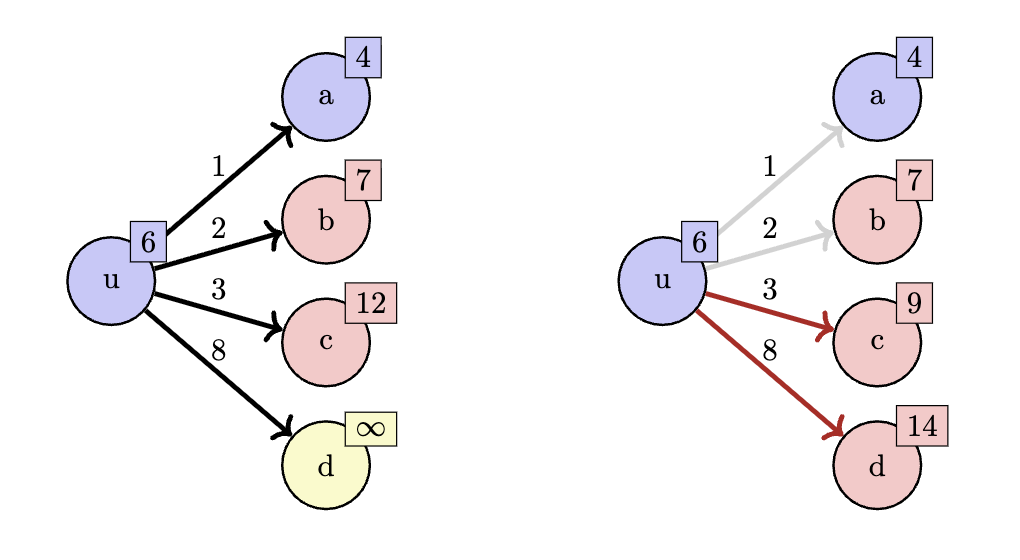
\includegraphics[scale=0.7]{d_greedy_update.png}
    \caption{An example of updating the out-neighbours of a node using the steps described above.}
    \label{fig:dijkstra_greedy_update}
\end{figure}

\begin{lemma}{}{}
    Let $v_1,\dots,v_n$ be the order in which the nodes are added to $S$. Then,
    $$
        \delta(s, v_i) \leq \delta(s, v_j) \quad \text{for } 1 \leq i \leq j \leq n \text{ and } d_s[v_i] = \delta(s, v_i) \text{ in iteration i.}
    $$
\end{lemma}

In simple terms, this lemma proves why Dijkstra's algorithm never has to change its mind. $S$ is the "settled set". These are nodes where the algorithm is sure that we know the shortest paths to them. $v_1, \dots, v_n$ is the exact order in which we work out the shortest path for each of these nodes. $\delta(s, v_i)$ is the true, objective shortest distance between $s$ and $v_i$. $d_s[v_i]$ is our current estimated distance to node $v_i$.

The lemma claims that: if $v_i$ is added to $S$ before $v_j$, then the true shortest distance from $s$ to $v_i$ is smaller than the true shortest distance from $s$ to $v_j$.

It also states that at the exact moment when $v_i$ is added to $S$, its estimate $d_s[v_i]$ is exactly correct and identical to $\delta(s, v_i)$.

\begin{figure}[h] % [h] attempts to place the image "here"
    \centering
    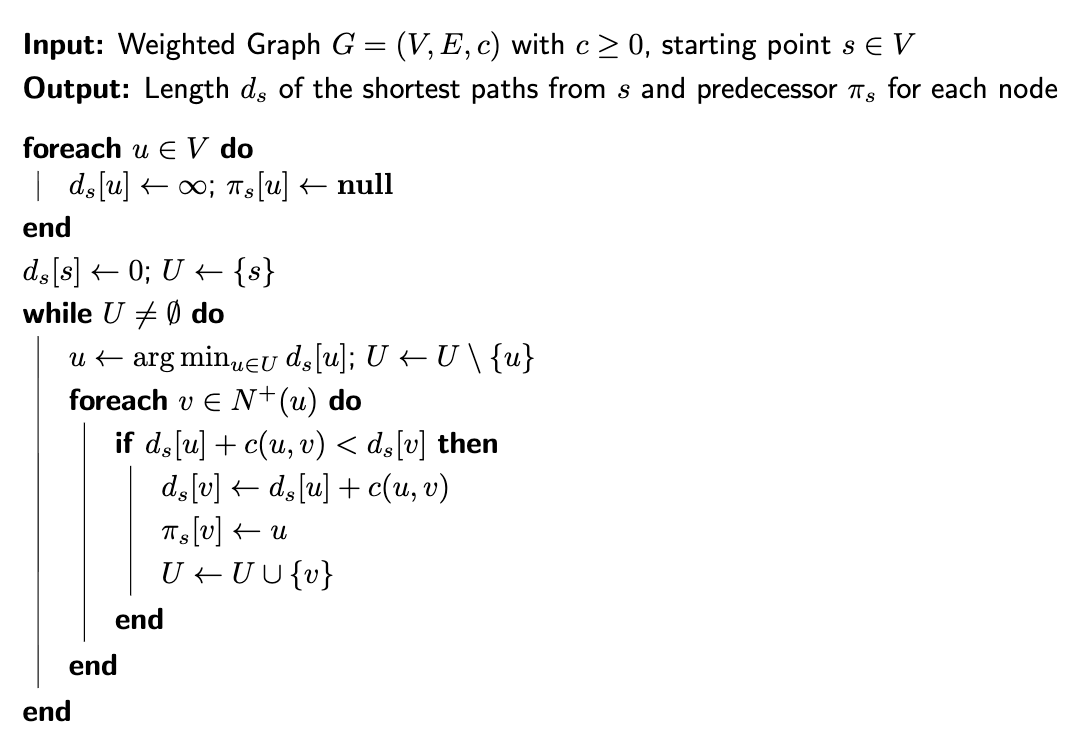
\includegraphics[scale=0.8]{d_pseudo.png}
    \caption{Pseudocode for Dijkstra's algorithm}
    \label{fig:dijkstra_pseudocode}
\end{figure}

\begin{notebox}{Data structure for $U$}{}
    We store $U$ in a min heap. This is because we need to be able to insert, as well as extract the minimum.

    In order to update priorities, we use \textbf{lazy deletion}. When we want to decrease the priority of a node $k$ from $p$ to $p' < p$, we leave the element $(p, k)$ untouched and add an additional element $(p', k)$ to the heap. When a node is extracted from the min heap from the first time, (with its smallest priority), we can mark it as deleted. Then, when we next encounter the node with a larger priority, we can ignore it and move to the next minimum.
\end{notebox}

\begin{figure}[h] % [h] attempts to place the image "here"
    \centering
    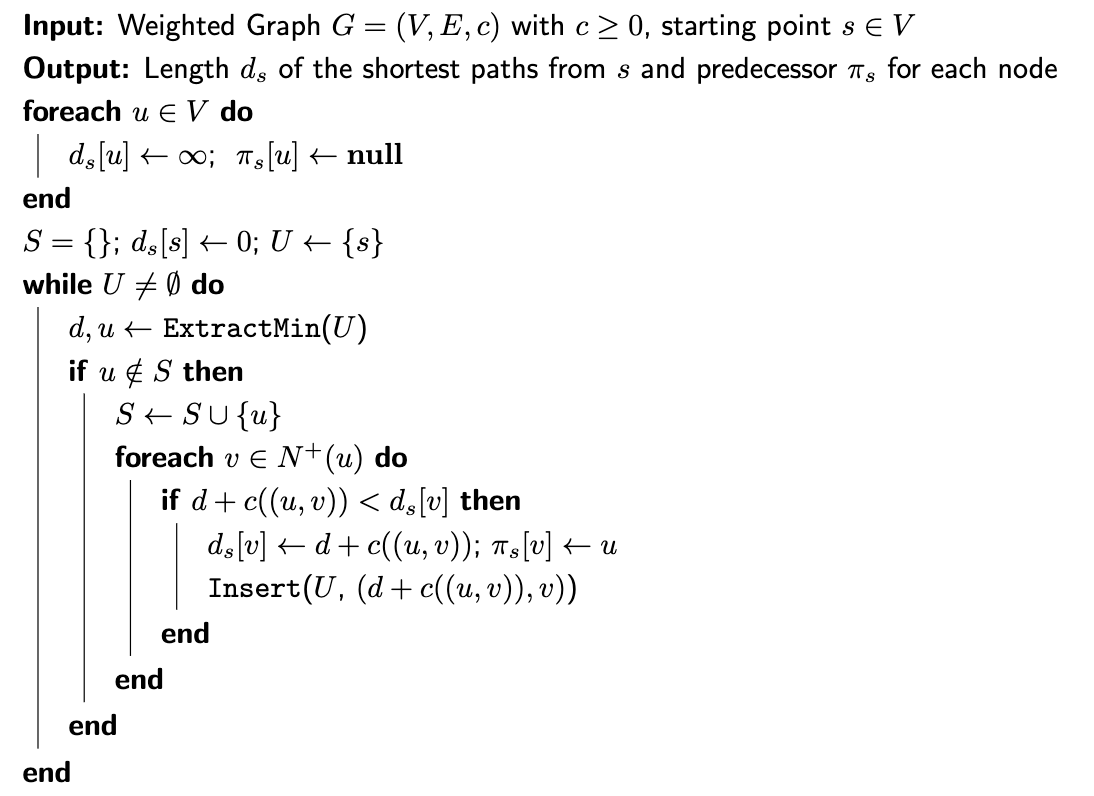
\includegraphics[scale=0.8]{d_pseudo_lazy_d.png}
    \caption{Pseudocode for Dijkstra's algorithm with lazy deletion}
    \label{fig:dijkstra_pseudocode_lazy_d}
\end{figure}

\subsection{$\text{A}^*$ Algorithm: Dijkstra with a heuristic}
If we already know where the goal is, then why bother exploring nodes which go in the wrong direction? This is the idea of the $\text{A}^*$ algorithm, we introduce a heuristic function. A possible choice for the heuristic is the Manhattan distance to the goal. Below is the pseudocode for $\text{A}^*$:

\begin{figure}[h] % [h] attempts to place the image "here"
    \centering
    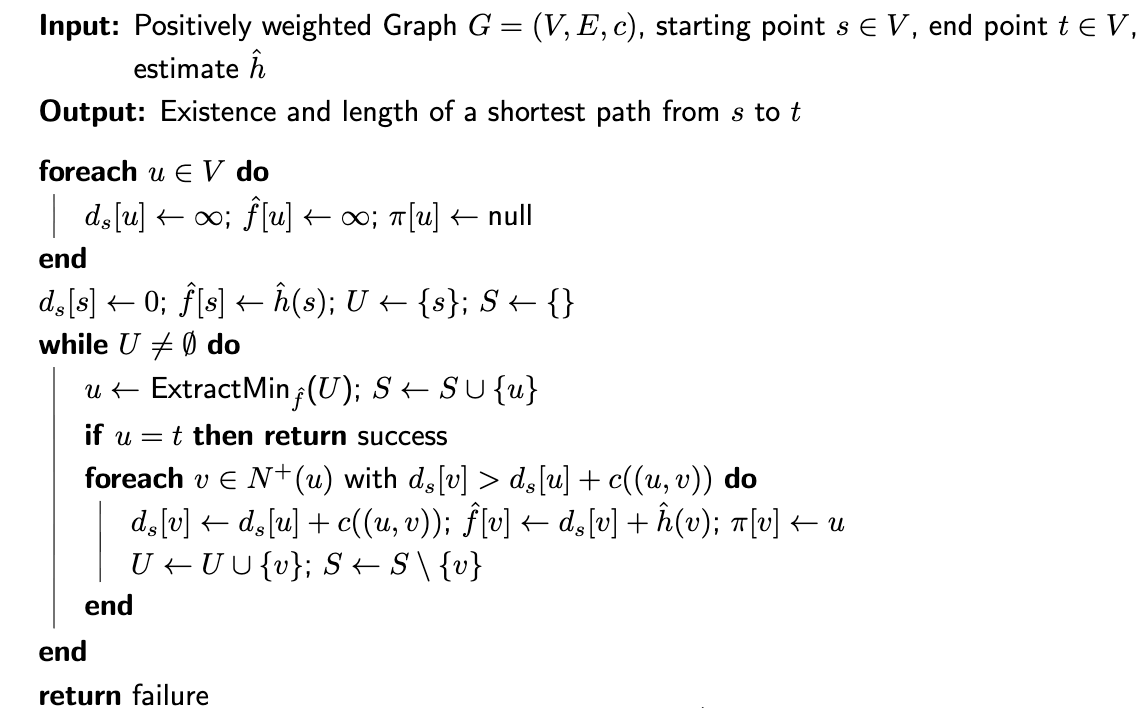
\includegraphics[scale=0.7]{a_star_pseudo.png}
    \caption{Pseudocode for $\text{A}^*$}
    \label{fig:a_star_pesudo}
\end{figure}

Let us now introduce properties of the heuristic function $\hat{h}$.

\begin{definition}{Optimistic heuristic}{}
    A heuristic $\hat{h}$ is optimistic, if
    $$
        \hat{h}(v) \leq \delta(v, t)
    $$

    where $\delta$ is the true shortest distance.
\end{definition}

\begin{definition}{Monotone heuristic}{}
    A heuristic $\hat{h}$ is monotone, if
    $$
        \hat{h}(u) \leq c((u, v)) + \hat{h}(v)
    $$
    holds for all $(u, v) \in E$.
\end{definition}

\begin{lemma}{}{}
    If $\hat{h}$ is optimistic, then $\text{A}^*$ terminates with the correct result, namely the shortest path from $s$ to $t$.
\end{lemma}

\begin{notebox}{Conclusion on heuristics}{}
    If $\bar{h}$ is \textbf{optimistic} and \textbf{monotone}, then the $\text{A}^*$ algorithm is correct and efficient. In practice, if underestimates are easy to compute (e.g. the distance as the crow flies), this can lead to drastic improvement of Dijkstra's algorithm.
\end{notebox}

\end{document}